\section{Structure of the source code}

\subsection{Microservices}
Here the code regarding the microservices architecture is explained. \\
The source code that meets the requirements mentioned above has been organized in the following way: for each microservices a project
has been set up. 
Indeed, when dealing with this type of architecture, one should think of a microservice
as a project that should me as much independent as possible from the others: this is the reason that stands behind the choice that has been
made. 
Of course, in this way, it is possible to easily generate the single jars that will be deployed, when necessary, with, as mentioned
in the design document, dockers. Therefore, the following projects are present: API gateway, service registry, group individual request
service, individual request service and share data service. 
As one may notice, the one containing the set up of the API gateway also accesses all the information related with the accounts, and, therefore, authentication and authorization functions are coded here.
In the following sections the structure of the single projects are analyzed. 

\subsubsection{API Gateway}
In the figure ~\ref{fig:pkgapigateway}, it is shown the root of the project structure. An analysis 
of the various elements follows below the figure. 
\begin{figure}[H]
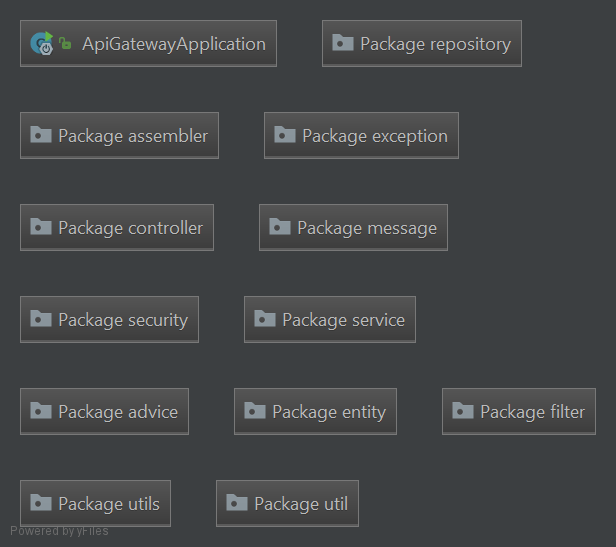
\includegraphics[width=\linewidth]{images/PackageApigateway.png}
\caption{ API gateway }
\label{fig:pkgapigateway}
\end{figure}

\begin{itemize}
\item Package repository: contains the JPA repository for accessing the persistent data necessary to this
service. 
In particular information regarding the accounts of users and third party customers are present. For what concerns the third party customers,
since they can register both as private and as related with a company the following repositories are present: company details, private
details, third party customers and users. An additional repository is present, and it accesses information regarding the API. Indeed, all
the accessible APIs that are available are stored in a database, in order to provide access control. For better specifying this choice, 
one may consider the fact that it is not necessary to search on the service registry non-existing API or to forward requests that can
be already classified as rejected (e.g. user A that is trying to access an API available only for third party customers)
\item Package assembler: this class contains components useful to build HATEOAS resources of entities that are returned to clients, adding
hypermedia contents
\item Package exception: this contains the custom exceptions defined during the development
\item Package controller: contains the controller that defines the APIs that regards the management of the users and third party customer
accounts. From here, it is possible to access the business functions that regards the account (e.g. login, logout, registration). Inside here,
controller are split into secure and public controllers: the public one are accessible to everyone, while for accessing the secured ones,
it is necessary to perform the log in
\item Package message: it provides the functions of communicating with other microservices, by means of RabbitMQ. In particular, three
subpackages are present here. The package publisher contains classes that helps in publishing the events of creation of new accounts to other
other services. The package protocol defines a way of communicating the interested pieces of information, and, finally the configuration
package specifies the configuration settings needed to convert object from JSON (and viceversa) during the exchange of data, and also
the Rabbit queues  
\item Package security: contains the main features that have been introduced above regarding the security 
\item Package service: contains the services that implements the business functions of the account service, with all the APIs that it exposes.
The interfaces present here map the component interfaces of the account service
\item Package advice: this encompasses the handling of server side exceptions in order to show to clients useful messages without exposing
the structure of the project and low level errors
\item Package entity: here classes that are mapped to the databases are present   
\item Package filter: it includes filters that the API gateway applies during the management of "external" requests (i.e. requests that
need to be processed by other services). In particular, it is further subdivided into three packages: pre, route and post. In this case, the
pre filter that is present perform access control on the external API that is being requested, the route filter is a translation filter
that adds header in order to identify the clients in the other microservices, and the post filter fixes the hypermedia content that is sent
as a response to the original request
\item Package util: various utility needed in the development
\end{itemize}

The routes to the other microservices available are present in the application.properties file.
Here it follows a list of the API available:
\begin{itemize}

\item /public/users/authorize \\
This requires two request parameters, that are user name and password. This API is necessary to login the users.
The method is POST.

\item /public/users/\{ssn\} \\
This is the entry point for registering a new user. Here, ssn is a path variable that specifies the social security number
of the user that will register. A request body that specifies the necessary fields of the JSON are specified in the user entity. \\
Here is reminded that one should check the needed fields paying attention also to the defined JSON views defined. \\
This holds also for the other methods in which a request body is needed. \\
The method is POST.


\item /public/thirdparties/authorize \\
This requires two parameters, that are email and password. This API is necessary to login the third party customers. 
The method is POST.

\item /public/thirdparties/companies is necessary to register a third party customer that is related with a company. \\
A request body is needed to specify all the information related to that customer.
The method is POST.

\item /public/thirdparties/privates is necessary to register a third party customer that is not related with a company.
A request body is needed to specify all the information related to that customer.
The method is POST.

\item /users/info returns the information of the user that is accessing that API 
The method is GET.

\item /users/logout performs the logout of a user from the system
The method is POST.

\item /thirdparties/info returns the information of the third party customer that is accessing the method
The method is GET.

\item /thirdparties/logout performs the logout of a third party customer from the system 
The method is POST.

\end{itemize}


\subsubsection{Service registry}
The project of the service registry is almost empty, no package is present, but just an application class is present, annotated with 
@EnableEurekaServer. The configuration of the service registry is set in the application.properties file.

\subsubsection{Group request service}
In the next figure, the package diagram of the group request project is shown ~\ref{fig:pkggrouprequest}. \\
The same comments hold here except for the fact that the business function mapped in the component interfaces are the one regarding
the group request service. 

\begin{figure}[H]
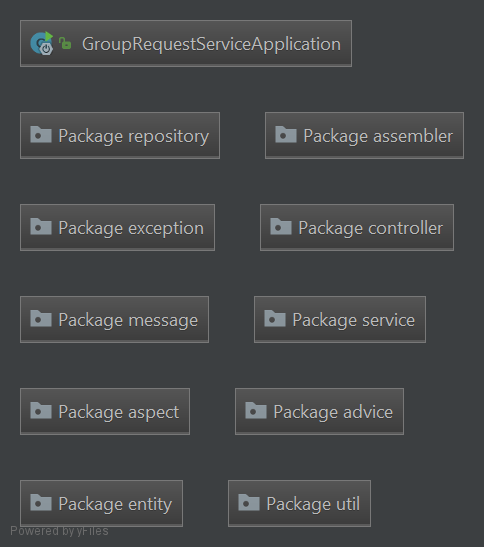
\includegraphics[width=\linewidth]{images/PackageGrouprequestservice.png}
\caption{ Group request service }
\label{fig:pkggrouprequest}
\end{figure}

Here it follows a list of the API available:
\begin{itemize}

\item /grouprequestservice/grouprequests/id/\{id\} \\
It retrieves the information related with the group request specified by the id in the
path variable. 
The method is GET.

\item /grouprequestservice/grouprequests/thirdparties \\
It collects all the group requests related with the third party that is accessing the method. 
The method is GET.

\item /grouprequestservice/grouprequests/thirdparties \\
This adds a new group requests. It requires a request body that contains all the details of the group
request that will be added.
The method is POST.

\end{itemize}

The prefix /grouprequestservice is necessary in order to access the APIs from the API gateway. 
Note, that by inspecting the controller, the prefix won't be shown at all: this is because the API gateway does this translation 
and mapping autonomously. Instead, one may notice some requested headers: they are added at runtime by the gateway, and so the client
don't have to specify them, and, if it does, they will be overwritten. \\
This comment holds, as well, for all the other microservices.


\subsubsection{Individual request service}
Here it follows the package diagram of the individual request service project ~\ref{fig:pkgindividualrequest}. 
As one may notice, the structure is very similar to the one explained in the api gateway project. 
Of course, here, the controllers provide access to the APIs that regards the individual request service. 
The business functions of this project are present in the  service package, and the interfaces that are present, 
are mapped with the component interfaces of the Design document. \\
Another difference w.r.t. the API gateway that is worth to point out is that here the package message contains also a subpackages that
defines listeners: these are charged of listening to new events that are forwarded from RabbitMQ. 

\begin{figure}[H]
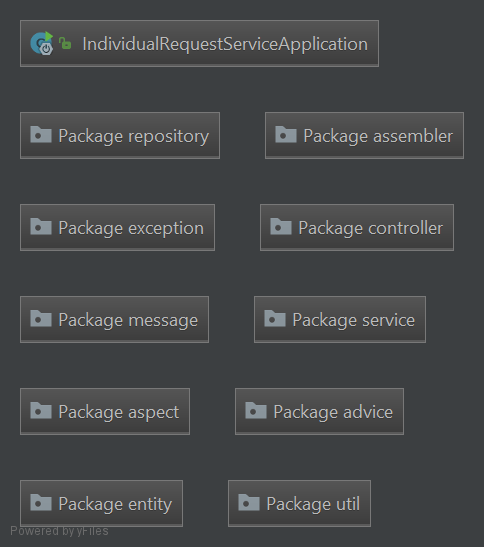
\includegraphics[width=\linewidth]{images/PackageIndividualrequestservice.png}
\caption{ Individual request service }
\label{fig:pkgindividualrequest}
\end{figure}

Here it follows a description of the available API:
\begin{itemize}
\item /individualrequestservice/requests/id/\{id\} \\
This retrieves an individual request identified by means of a certain id. 
The method is GET.

\item /individualrequestservice/requests/users \\ 
This retrieves the pending requests of the user that is accessing the method. 
The method is GET.

\item /individualrequestservice/requests/thirdparties \\ 
This retrieves the requests performed by the third party customer that is accessing the method.
The method is GET.

\item /individualrequestservice/requests/\{ssn\} \\
This adds a new individual request toward the user specified in the path variable.
A request body specifies the information requested to define the individual request.
The method is POST. 

\item /individualrequestservice/responses/requests/{requestID} \\
It is used in the case in which the user that is accessing the method
sends a response to the request identified by requestID in the path variable.

\item /individualrequestservice/responses/blockedThirdParty/thirdparties/{thirdParty} \\
It is used in the case in which the user that is accessing the method blocks the third party identified by the id specified in the path variable
\end{itemize}

\subsubsection{Share data service}
The structure of the share data service, as shown by the following picture, is also very similar to the previous ones 
~\ref{fig:pkgsharedata}.

\begin{figure}[H]
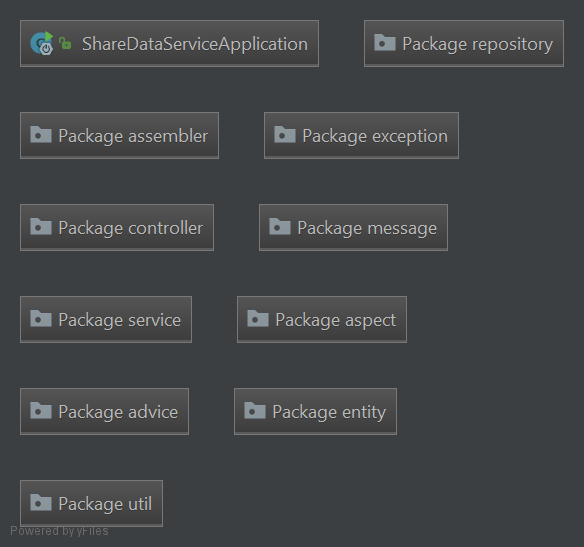
\includegraphics[width=\linewidth]{images/PackageSharedataservice.png}
\caption{ Share data service }
\label{fig:pkgsharedata}
\end{figure}

However, it is important to point out the structure of the code that manages the personalized query specified by the group requests on 
anonymized data. Basically, the custom query is realized with the help of QueryDSL, a sort of unified library to make queries; this choice comes from a limitation of Spring JPA: the impossibility to make union with dynamic queries. Therefore, after researches of other libraries supporting JPA, the best one and mostly supported by the community was QueryDSL which offers a method to makes JPA SQL queries. First of all it is necessary to say that JPA creates connection between objects of classes  and tuples of the DB; this has great advantages when it comes to use only JPA, but mixing it with other methods of retrieving data such as raw SQL queries could introduce some inconsistency. But thanks to JPA SQL queries it was possible to avoid this problem. In conclusion, the custom query is generally something with this simplified template:
\begin{itemize}
\item SELECT AGG\_OP(Column) FROM User JOIN ON Union(HealthData dynamic filtered, PositionData dynamic filtered) WHERE (sameSSN) AND "other filters of User table"
\end{itemize}
  
Here it follows a list of the main API that have been developed in the project, and that are located
within the various microservices.
It is possible to find these mapping in the controller packages. \\
The methods are expressed from a client point of view: for example, takes into consideration the methods that starts with s 

Here it follows a description of the available API

\begin{itemize}
\item /sharedataservice/dataretrieval/individualrequests/\{request\_id\} \\
This method retrieves the data related to the individual request identified by the path variable. The method is GET.

\item /sharedataservice/dataretrieval/grouprequests/\{request\_id\} \\
This method retrieves the data related to the group request identified by the path variable. The method is GET.

\item /sharedataservice/dataretrieval/users \\
This method retrieves the own data of the user. In this case, two request parameters
are necessary in order to specify an interval of time that involves the interested data.
The method is GET.

\item /sharedataservice/datacollection/healthdata \\
This allows the user to send data regarding the health status to the system. The method is POST.
A request body that specifies the data is required.

\item /sharedataservice/datacollection/positiondata \\
This allows the user to send data regarding his position data to the system. The method is POST.
A request body that specifies the data is required.

\item /sharedataservice/datacollection/clusterdata
This allows the user to send cluster of data (both health and position data). The method is POST.
A request body that specifies the data is required.

\end{itemize}



\subsection{Mobile code}

\subsubsection{Data4Help}

\subsubsection{AutomatedSOS}
The service regarding AutomatedSOS is completely developed to work locally on the smartphone of the user to achieve a high availability. Of course, it also has to have a high reliability, therefore, it is designed to be testable as possible. The project is subdivided in different packages:
\begin{itemize}
	\item bluetooth: this package deals with the communication between the other device collecting health data. Basically it is based on a BluetoothServer class which waits for a connection; once the connection is established, a SocketHandler object is instantiated and it waits for specific messages which will be forwarded to a HealthDataCallback that is responsible to save the health data and ask for a call if necessary.
	\item health: here, there is the HealthService that deals with the notification and starting the bluetooth server and other objects. Another important class is the HealthServiceHelper which is used by HealthDataCallback to be able to call the service.
	\item util: other utility classes such as HealthDataInspector which checks if a specific health data is dangerous for the user or not.
	\item exception: all the exception that could happen during the chain of action to reach a call.
\end{itemize}

